\textbf{\underline{OZ 6 - Magnetische inductie en de wet van Faraday - Oefening 4:}}
\vspace{0.5cm}

    Bepaal de emf geïnduceerd in een vierkante lus waarbij de lus in rust blijft en een stroom in de rechte draad gegeven is door $I(t) = 15.0\sin(2500t)$ A met $t$ de tijd in seconden. De afstand $a$ is $12.0$ cm, en $b$ is $15.0$ cm.

    \begin{center}
        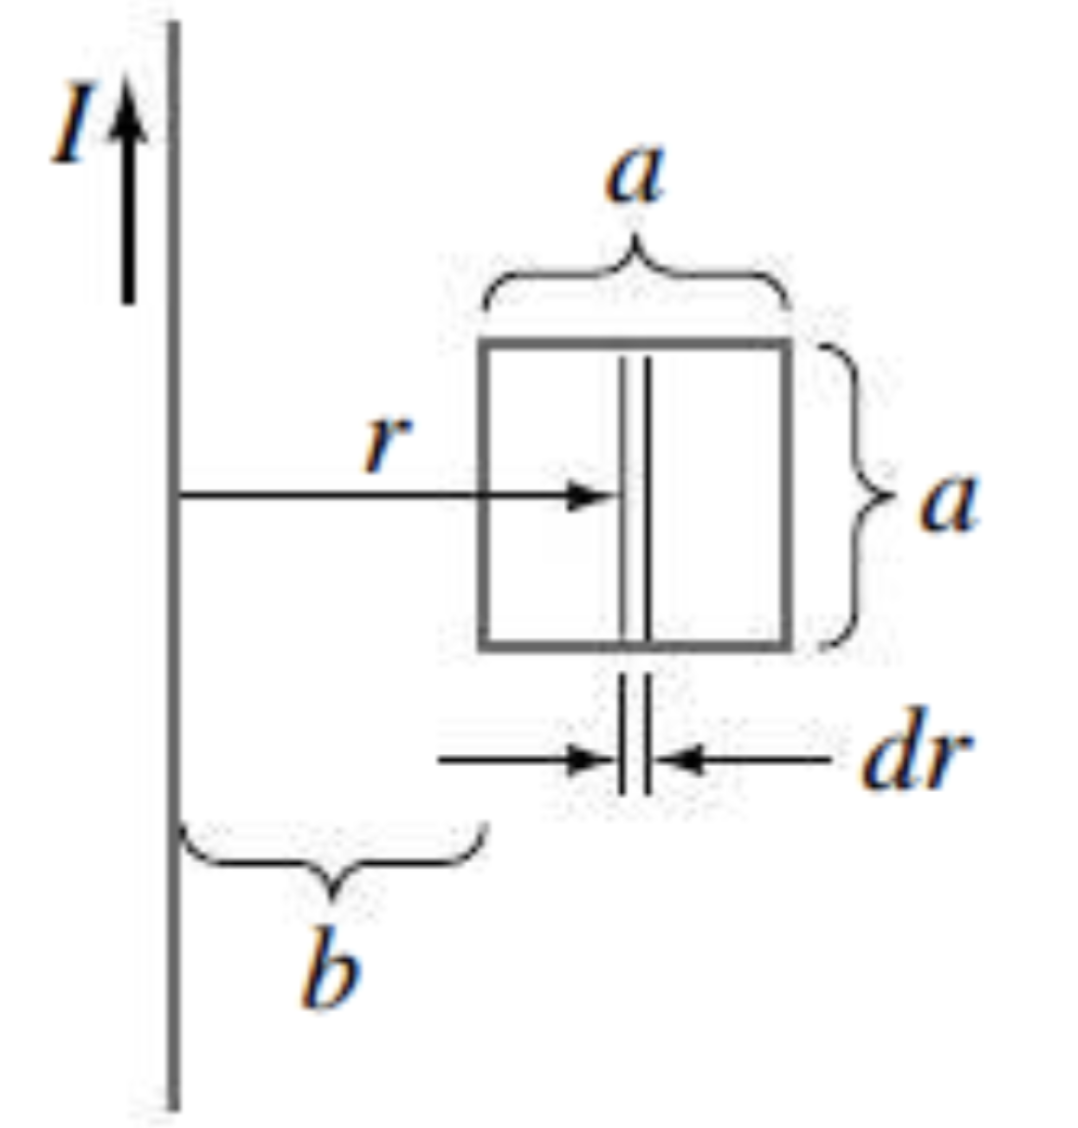
\includegraphics[scale = 0.2]{oz06/resources/Oz6Oef4.png}
    \end{center}

    \begin{description}[labelwidth=1.5cm, leftmargin=!]
        \item[Geg. :] $I(t) = 15.0\sin(2500t)$ A, $a = 12.0 \cdot 10^{-2}$ m, $b = 15.0 \cdot 10^{-2}$ m
        \item[Gevr. :] $\mathcal{E}_{\text{ind}}$
        \item[Opl. :]
            We kunnen de wet van Faraday gebruiken om de geïnduceerde emf te vinden
            \begin{align*}
                \mathcal{E}_{\text{ind}}(t) 
                    &= - \frac{d}{dt} \left( \int \vec{B} \cdot d\vec{A} \right) \\
                    &= - \frac{d}{dt} \left( \int B dA \right) \\
                    &= - \frac{d}{dt} \left( \int \frac{\mu_0 I(t)}{2\pi r}adr \right) \\
                    &= - \frac{dI(t)}{dt} \left( \frac{\mu_0a}{2\pi}\ln\left(1+\frac{a}{b}\right)\right) 
            \end{align*}
            wat ons geeft
            \begin{equation*}
                \mathcal{E}_{\text{ind}}(t) = 5.30 \cos(2500t) \cdot 10^{-4} \ \text{V}.
            \end{equation*}
            als we het gegeven invullen.
    \end{description}

\vspace{1cm}